\documentclass{article}
\usepackage[margin=1in]{geometry}
\usepackage{tikz}
\usetikzlibrary{arrows.meta,calc,positioning,patterns}

\pagestyle{empty}

\begin{document}

    \begin{center}
        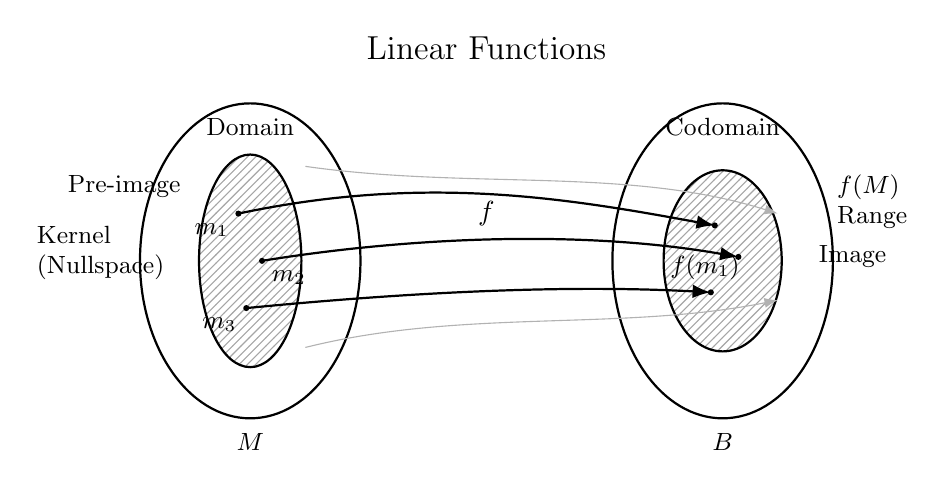
\begin{tikzpicture}[
            >=Latex,
            every node/.style={font=\small},
            set/.style={draw, thick},
            inner/.style={draw, thick, pattern=north east lines, pattern color=gray!70},
            map/.style={->, thick}
        ]

% Title
            \node[font=\large] at (5,4.2) {Linear Functions};

% --- Domain (left) ---
            \node at (2,3.2) {Domain};

% Outer oval M
            \draw[set] (2,1.5) ellipse (1.4 and 2.0);
            \node at (2,-0.8) {$M$};

% Inner shaded oval = kernel
            \draw[inner] (2,1.5) ellipse (0.65 and 1.35);

% Labels on left
            \node[align=left] at (0.1,1.6) {Kernel\\(Nullspace)};
            \node[align=left] at (0.4,2.45) {Pre-image};

% Sample points in domain
            \fill (1.85,2.1) circle (1.1pt) node[below left] {$m_1$};
            \fill (2.15,1.5) circle (1.1pt) node[below right] {$m_2$};
            \fill (1.95,0.9) circle (1.1pt) node[below left] {$m_3$};

% --- Codomain (right) ---
            \node at (8,3.2) {Codomain};

% Outer oval B
            \draw[set] (8,1.5) ellipse (1.4 and 2.0);
            \node at (8,-0.8) {$B$};

% Inner shaded oval = image/range
            \draw[inner] (8,1.5) ellipse (0.75 and 1.15);

% Labels on right
            \node[align=left] at (9.9,2.25) {$f(M)$\\Range};
            \node[align=left] at (9.65,1.55) {Image};

% Sample points in image
            \fill (7.9,1.95) circle (1.1pt) node[below left,label=270:$f(m_1)$] {};
            \fill (8.2,1.55) circle (1.1pt);
            \fill (7.85,1.10) circle (1.1pt);

% Label f over arrows
            \node[font=\normalsize] at (5,2.1) {$f$};

% --- Mapping arrows ---
            \draw[map] (1.85,2.1) .. controls (4.2,2.6) and (6.0,2.3) .. (7.9,1.95);
            \draw[map] (2.15,1.5) .. controls (4.0,1.8) and (6.2,1.9) .. (8.2,1.55);
            \draw[map] (1.95,0.9) .. controls (4.0,1.1) and (6.0,1.2) .. (7.85,1.10);

% Extra faint arrows to mimic the sketch
            \draw[->, thin, gray!60] (2.7,2.7) .. controls (4.8,2.4) and (6.8,2.7) .. (8.7,2.1);
            \draw[->, thin, gray!60] (2.7,0.4) .. controls (4.7,0.9) and (6.7,0.6) .. (8.7,1.0);



        \end{tikzpicture}
    \end{center}

\end{document}